
\documentclass[12pt]{beamer}
\usetheme{Warsaw}

\definecolor{myblue1}{RGB}{35,119,189}
\definecolor{myblue2}{RGB}{95,179,238}
\definecolor{myblue3}{RGB}{129,168,207}
\definecolor{myblue4}{RGB}{26,89,142}

\setbeamercolor*{structure}{fg=myblue1,bg=blue}
\setbeamercolor*{palette primary}{use=structure,fg=white,bg=structure.fg}
\setbeamercolor*{palette secondary}{use=structure,fg=white,bg=structure.fg!75!black}
\setbeamercolor*{palette tertiary}{use=structure,fg=white,bg=structure.fg!50!black}
\setbeamercolor*{palette quaternary}{fg=black,bg=white}

\setbeamercolor*{item projected}{fg=red,bg=myblue3!80}
\setbeamercolor*{block title example}{fg=white,bg=myblue4}
\setbeamercolor*{frametitle}{fg=black}

\setbeamertemplate{blocks}[rounded][shadow=true]

\makeatletter
\pgfdeclarehorizontalshading[frametitle.bg,frametitle right.bg]{beamer@frametitleshade}{\paperheight}{%
	color(0pt)=(myblue2);
	color(\paperwidth)=(white)}

\defbeamertemplate*{footline}{mysplit theme}
{%
	\leavevmode%
	\hbox{\begin{beamercolorbox}[wd=.5\paperwidth,ht=2.5ex,dp=1.125ex,leftskip=.3cm plus1fill,rightskip=.3cm]{author in head/foot}%
			\usebeamerfont{author in head/foot}\insertshortauthor
		\end{beamercolorbox}%
		\begin{beamercolorbox}[wd=.5\paperwidth,ht=2.5ex,dp=1.125ex,leftskip=.3cm,rightskip=.3cm plus1fil]{title in head/foot}%
			\usebeamerfont{title in head/foot}\insertshorttitle\hfill
			\insertframenumber/\inserttotalframenumber\hspace*{0.5em}
	\end{beamercolorbox}}%
	\vskip0pt%
}
\makeatother

\usepackage[english]{babel}
\usepackage[utf8x]{inputenc}

\usepackage{xcolor}
\usepackage{color}
\definecolor{rscuro}{rgb}{0.75,0.0,0.0}
\definecolor{bscuro}{rgb}{0.0,0.2,0.5}

\usepackage{graphicx}
\graphicspath{{Presentation_images/}}                 								
\usepackage[font=small,format=hang]{caption}  										
\captionsetup{tableposition=top,figureposition=bottom,font=small, format=hang,labelfont={sf,bf}} 	
\usepackage{subfig}

\usepackage{eurosym}

\title[Study of French labour market and inequalities]{Study of French labour market and inequalities} 
\author{L. Insolia, J. Kim and G. Yeghikyan}
\institute{SNS \\
		   \vskip0.5cm\centering\small \textcolor{rscuro}{--- \emph{Midterm results} ---}}
\date{March 14, 2018}

\beamertemplatenavigationsymbolsempty

%\begin{document}
%	
%	\begin{frame}
%	\maketitle
%\end{frame}
%
%\section{Propositional Argumentation Systems}
%\subsection{Propositional Logic}
%\begin{frame}
%\frametitle{Logical consequences}
%\begin{itemize}
%	\item First.
%	\item Second.
%	\item Third.
%	\begin{exampleblock}{Entailment Relation}
%		\begin{itemize}
%			\item First.
%			\item Second.
%		\end{itemize}
%	\end{exampleblock}
%	\item Fourth.
%\end{itemize}
%\end{frame}
%
%\subsection{Argumentation Systems}
%\begin{frame}
%\frametitle{Logical consequences}
%\end{frame}
%\subsection{Probabilistic Argumentation Systems}
%\begin{frame}
%\frametitle{Logical consequences}
%\end{frame}
%
%\section{Argumentation Systems on Set Constraint Logic}
%\begin{frame}
%test
%\end{frame}
%
%\end{document}


\begin{document}
	
\begin{frame}
	
	\maketitle
\end{frame}


\section{Preview}

\subsection{Motivation}

\begin{frame}{\textcolor{bscuro}{Objectives}}
%	   What were the aims of your project, and what is the context – in terms of subject matter questions, and in terms of applicable statistical and computational tools.  				
	\begin{itemize}
		\item Structure of French labour market 
		\item Inequalities (in terms of salary): 
		\begin{itemize}
			\item ages 
			\item gender
			\item job categories
			\item spatial distribution
		\end{itemize}
		\item Firms' distribution
		\item Exploratory analyses
	\end{itemize}
\end{frame}
		

\subsection{Approach}

\begin{frame}{\textcolor{bscuro}{Methodology}}
%	  Description of the dataset (where is it from what is the information shared through this dataset, what year)and the variables that we have, what are the interesting features that we can use to study 
	INSEE data
	\begin{itemize}
		\item Population: age, sex and cohabitation mode
		\item Salary: job categories, age and sex (mean net salary per hour in \euro)
		\item Firms: number of firms for each size
		\item Geography: GPS location
	\end{itemize}
	for different geographical levels (communes, departments, \underline{towns}) in 2014
	
	
	\vskip1cm GitHub repo: \textcolor{bscuro}{\url{https://github.com/LucaIns/TSL}} % \\
%			  Kaggle: \textcolor{bscuro}{\url{https://www.kaggle.com/etiennelq/french-employment-by-town}}
\end{frame}
				

\section{Preliminary results}


\begin{frame}
	\centerline{\Huge\textcolor{bscuro}{What has been done so far \ldots}}		
\end{frame}


\begin{frame}{\textcolor{bscuro}{Pre-processing phase}}
	\begin{itemize}
		\item Population: restructured the dataset and created new features
		\item Firms: categorized firms' sizes into 4 categories
		\item Geography: retrieved the missing data using Google API
	\end{itemize}
\end{frame}


\subsection{Population}


\begin{frame}{\textcolor{bscuro}{Distribution of population per town}}
	%			\item insight to demographic profile for each town 
	%			\item age into three different categories: child, workforce and elderly
	%			\item sex and dependency ratios 
	\begin{figure}[!ht] 
		\centering
		\subfloat{{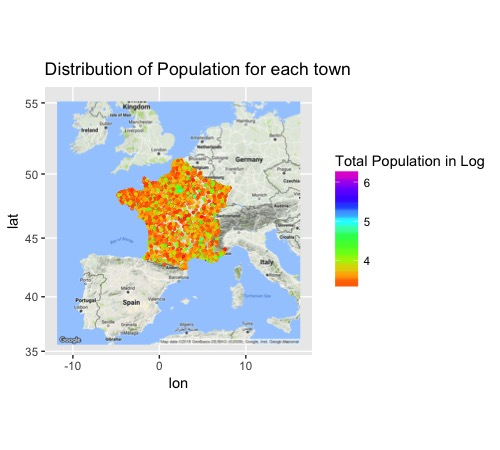
\includegraphics[width=0.55\textwidth]{DDis_pop.jpeg} }}
		\subfloat{{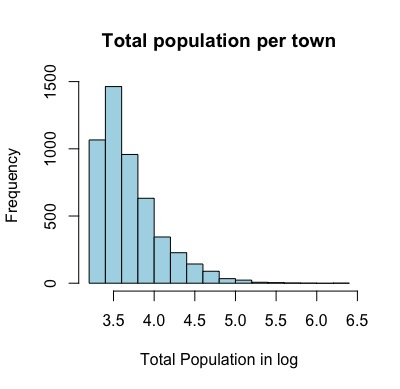
\includegraphics[width=0.5\textwidth]{tot_pop.jpeg} }}
	\end{figure}
\end{frame}

\begin{frame}{\textcolor{bscuro}{Population demographics}}
	\begin{figure}[!ht] 
		\centering
		\subfloat{{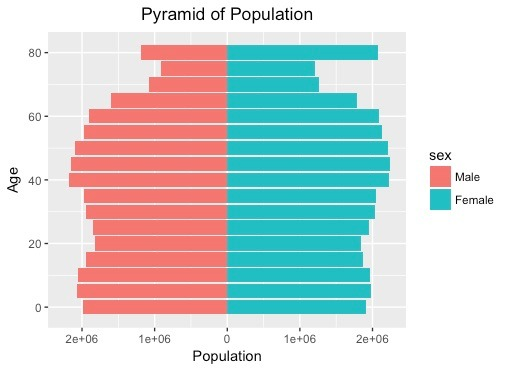
\includegraphics[width=0.6\textwidth]{pyramid_pop.jpeg} }}
		\subfloat{{\includegraphics[width=0.5\textwidth]{Aged.jpeg} }}
	\end{figure}
\end{frame}

\begin{frame}{\textcolor{bscuro}{PCA}}
\begin{figure}[!ht] 
	\centering
	\subfloat{{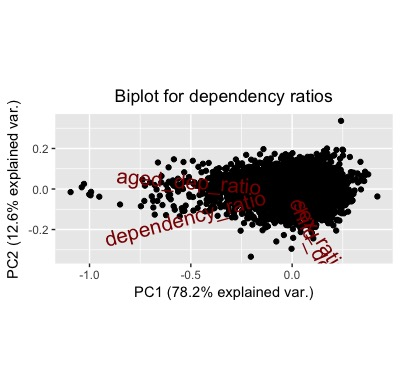
\includegraphics[width=0.6\textwidth]{Biplot_pop.jpeg} }}
\end{figure}
\end{frame}


\subsection{Salary} 


\begin{frame}{\textcolor{bscuro}{Inequality of salary}}	
	\begin{figure}[!ht] 
		\centering
		\subfloat{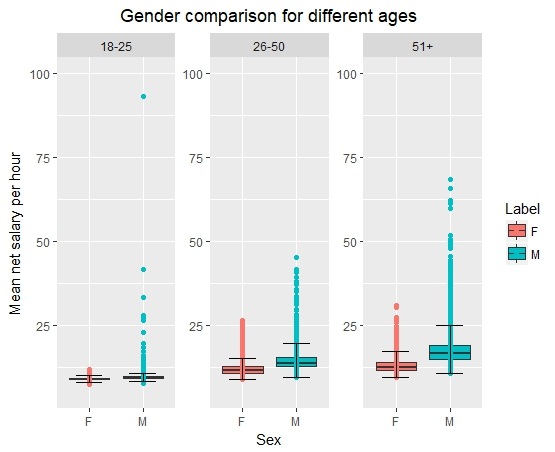
\includegraphics[width=0.5\textwidth]{boxplot_sex_age.jpeg}} 
		\subfloat{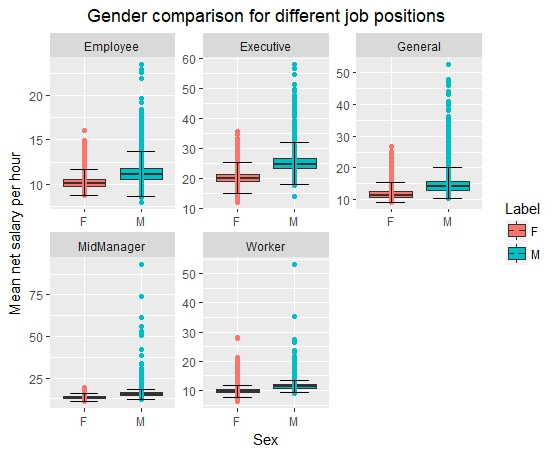
\includegraphics[width=0.5\textwidth]{boxplot_sex_job.jpeg}}
	\end{figure}
\end{frame}
	
	
\begin{frame}{\textcolor{bscuro}{Inequality of salary}}	
	\begin{figure}[!ht] 
		\centering
		\subfloat{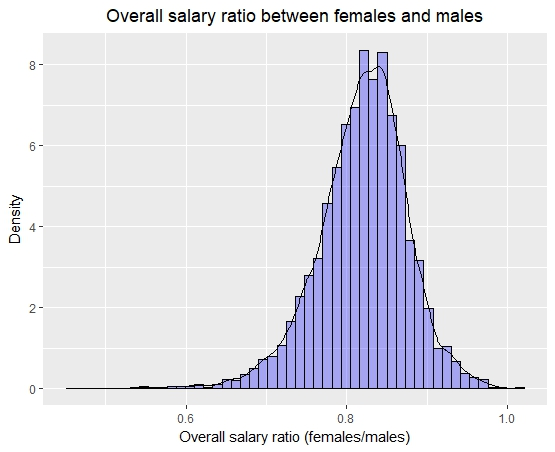
\includegraphics[width=0.5\textwidth]{hist_salary_ratio_general.jpeg}} 
		\subfloat{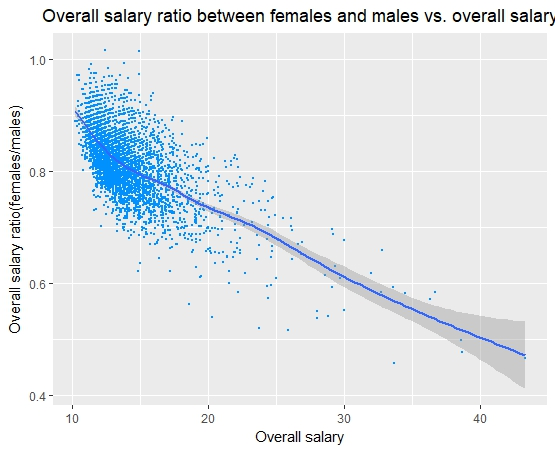
\includegraphics[width=0.5\textwidth]{scatter_salary_ratio_vs_general.jpeg}}
	\end{figure}
\end{frame}


\begin{frame}{\textcolor{bscuro}{Inequality of salary}}	
	\begin{figure}[!ht] 
		\centering
		\subfloat{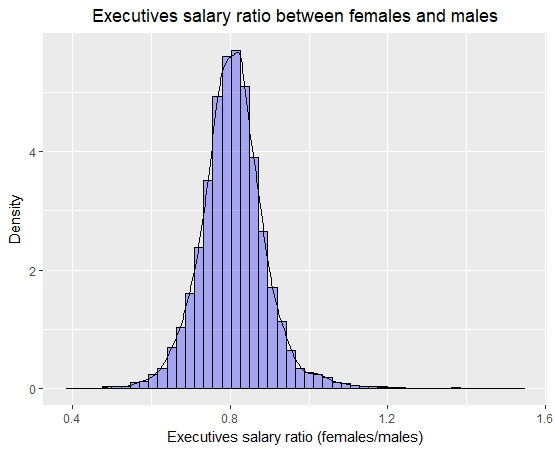
\includegraphics[width=0.5\textwidth]{hist_salary_ratio_executives.jpeg}} 
		\subfloat{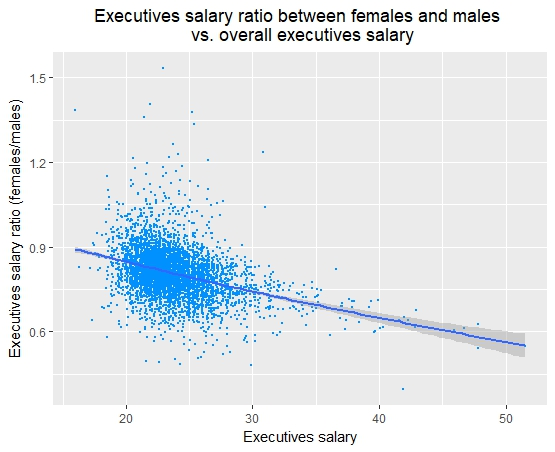
\includegraphics[width=0.5\textwidth]{hist_salary_ratioExec_vs_executives.jpeg}}
	\end{figure}
\end{frame}


\begin{frame}{\textcolor{bscuro}{Inequality of salary}}	
\begin{figure}[!ht] 
	\centering
	\subfloat{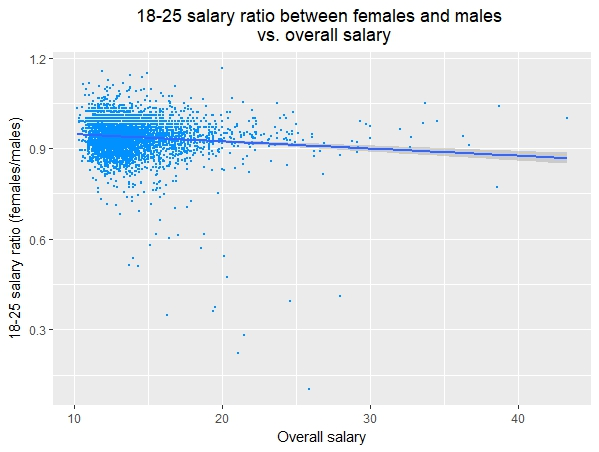
\includegraphics[width=0.5\textwidth]{scatter_salary_ratio_18_25_vs_general.jpeg}} 
	\subfloat{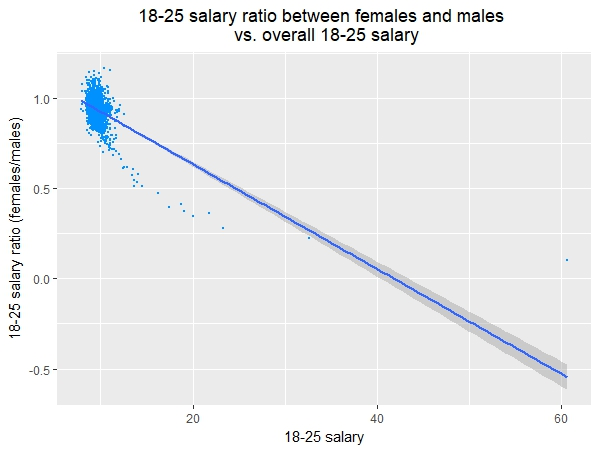
\includegraphics[width=0.5\textwidth]{scatter_salary_ratio_18_25_vs_general18_25.jpeg}}
\end{figure}
\end{frame}


\begin{frame}{\textcolor{bscuro}{Bivariate relations}}	
\begin{figure}[!ht] 
	\centering
	\subfloat{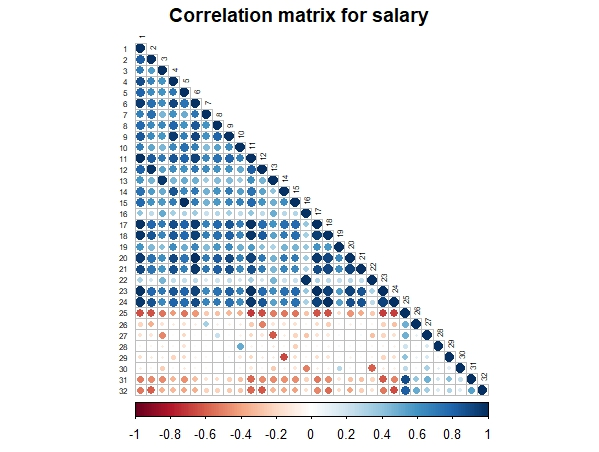
\includegraphics[width=0.5\textwidth]{correl_salary.jpeg}} 
	\subfloat{\includegraphics[width=0.5\textwidth]{scatter_salary.jpeg}}
\end{figure}
\end{frame}


\begin{frame}{\textcolor{bscuro}{ANOVA using sex, job, age and interaction effects}}
	\begin{figure}[!ht] 
		\centering
		\subfloat{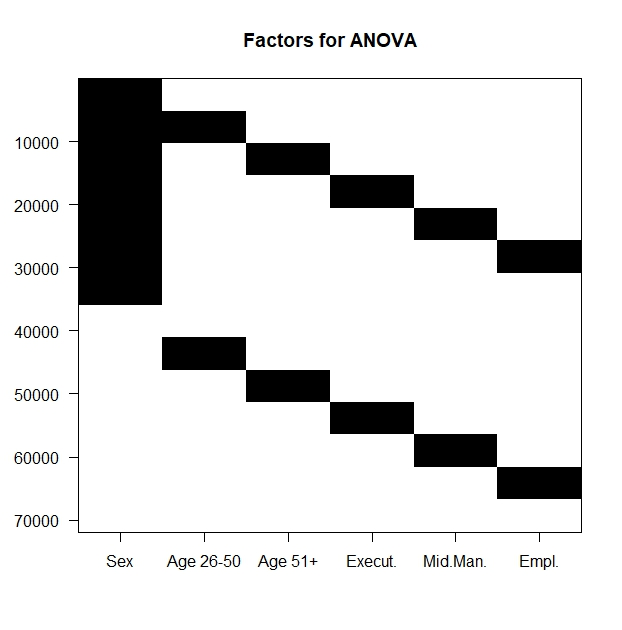
\includegraphics[width=0.5\textwidth]{ANOVA_factors.jpeg}} 
		\subfloat{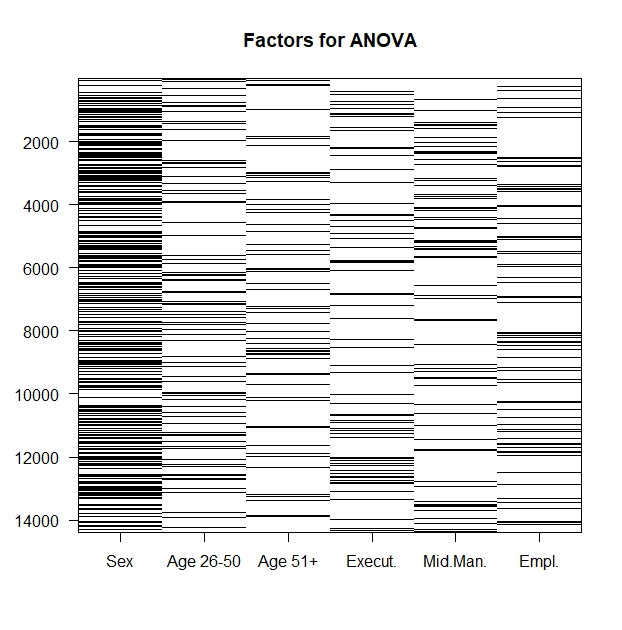
\includegraphics[width=0.5\textwidth]{ANOVA_factors_randomized.jpeg}}
	\end{figure}
\end{frame} 


\begin{frame}{\textcolor{bscuro}{ANOVA using sex, job, age and interaction effects}}
	\begin{figure}[!ht] 
		\centering
		\subfloat{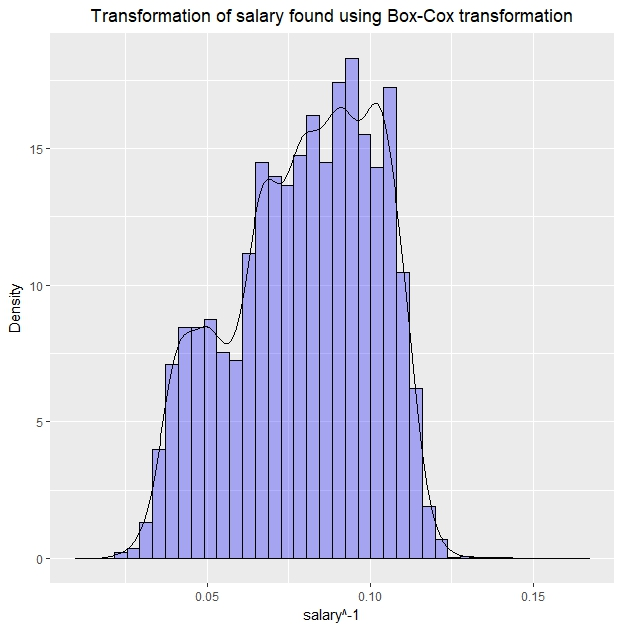
\includegraphics[width=0.6\textwidth]{ANOVA_dataY.jpeg}} 
	\end{figure}
\end{frame}

	
\begin{frame}{\textcolor{bscuro}{Prediction for young people using BSS }}
	\begin{figure}[!ht] 
		\centering
		\subfloat{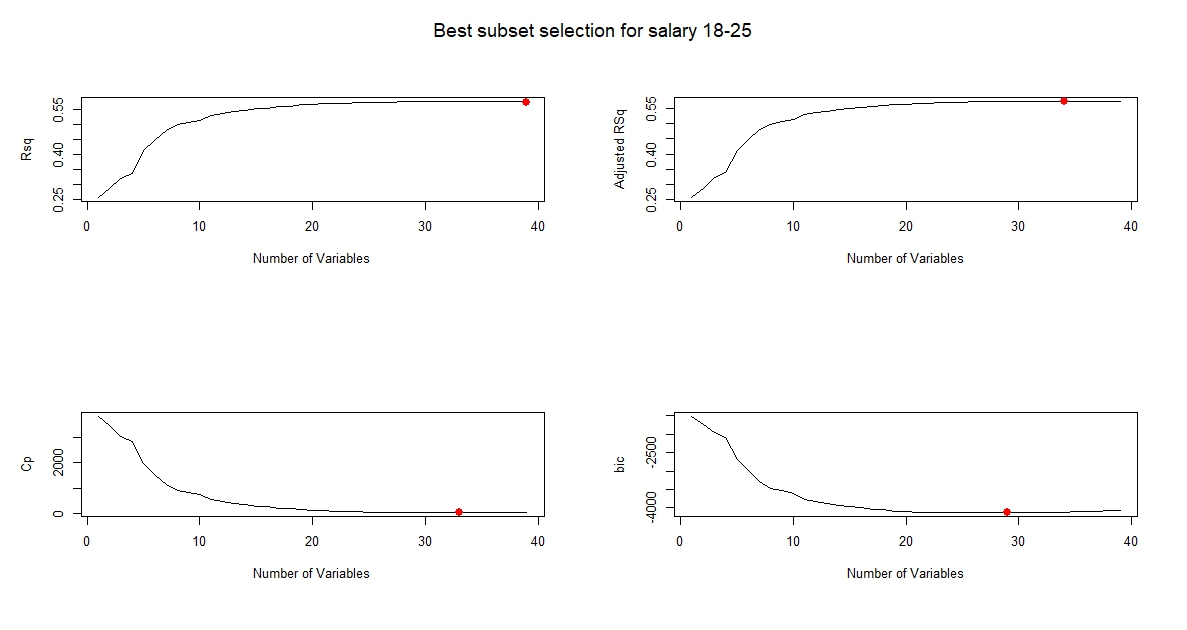
\includegraphics[width=0.6\textwidth]{bestsubsel_18_25.jpeg}} 
		\qquad
		\subfloat{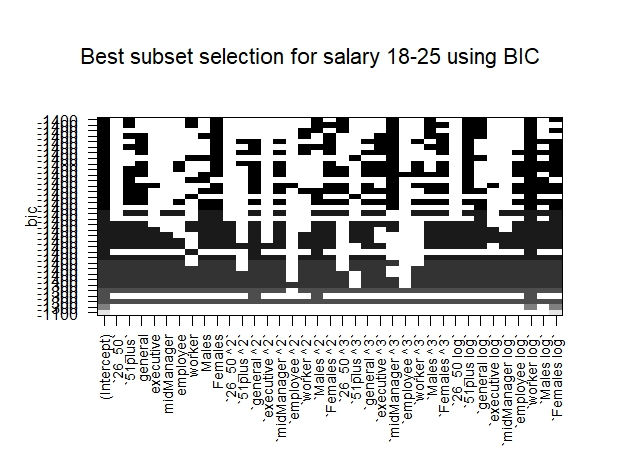
\includegraphics[width=0.5\textwidth]{bestsubsel_18_25_BIC.jpeg}}
	\end{figure}
\end{frame}

	
\begin{frame}{\textcolor{bscuro}{Elastic net and and 10-folds CV}}
	\begin{figure}[!ht] 
		\centering
		\subfloat{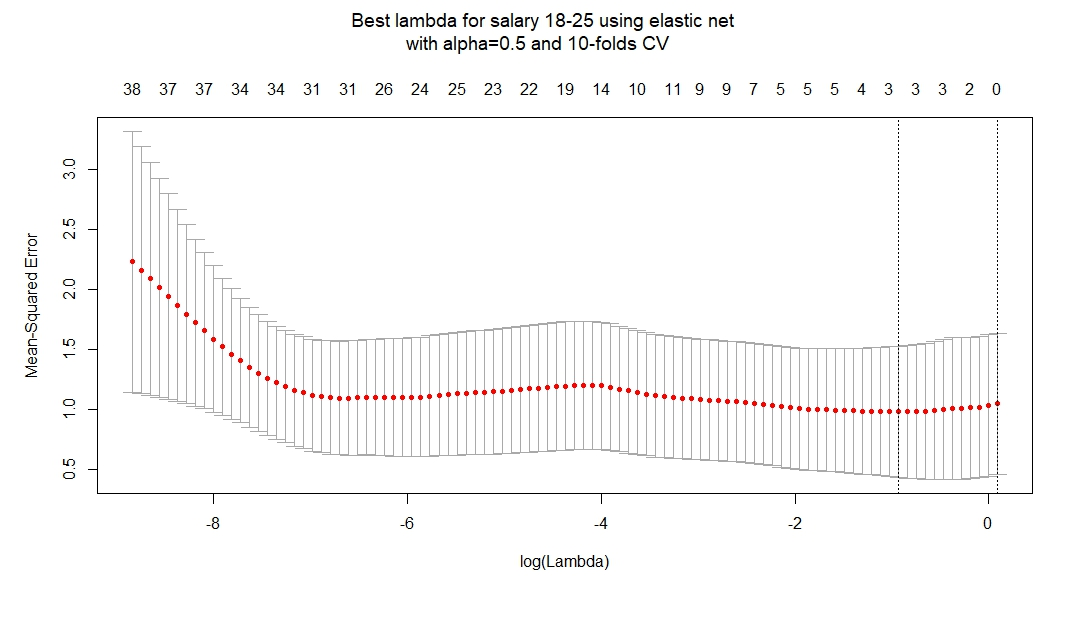
\includegraphics[width=0.9\textwidth]{elasticNet_10foldsCV.jpeg}} 
	\end{figure}
\end{frame}


\subsection{Firms}


\begin{frame}{\textcolor{bscuro}{Distribution of firms per town}}
	\begin{figure}[!ht] 
		\centering
		\subfloat{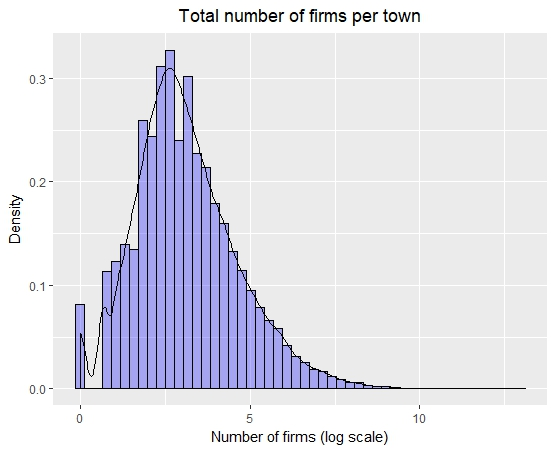
\includegraphics[width=0.5\textwidth]{hist_firms_total.jpeg}}
		\subfloat{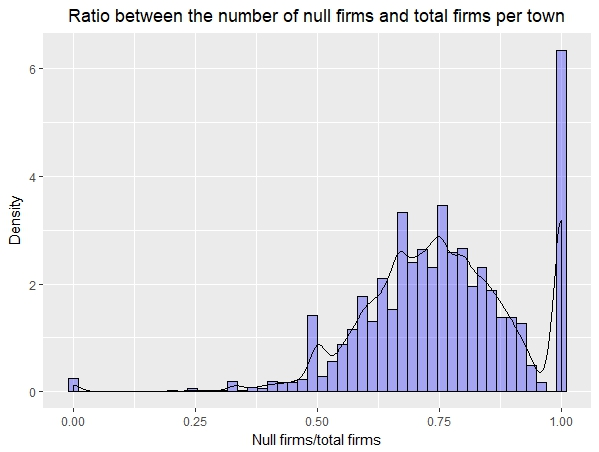
\includegraphics[width=0.5\textwidth]{hist_firms_ratio_null_total.jpeg}}
	\end{figure}
\end{frame}


\begin{frame}{\textcolor{bscuro}{Bivariate relations}}
\begin{figure}[!ht] 
	\centering
	\subfloat{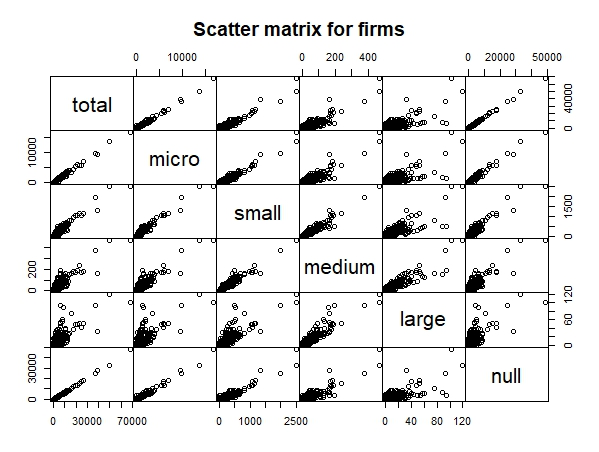
\includegraphics[width=0.5\textwidth]{scatter_firms.jpeg}}
	\subfloat{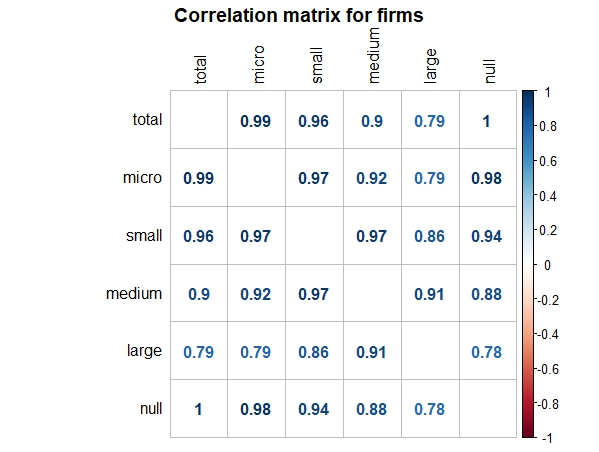
\includegraphics[width=0.5\textwidth]{corr_firms.jpeg}}
\end{figure}
Excluding Paris
\end{frame}


\begin{frame}{\textcolor{bscuro}{Bivariate relations}}
\begin{figure}[!ht] 
	\centering
	\subfloat{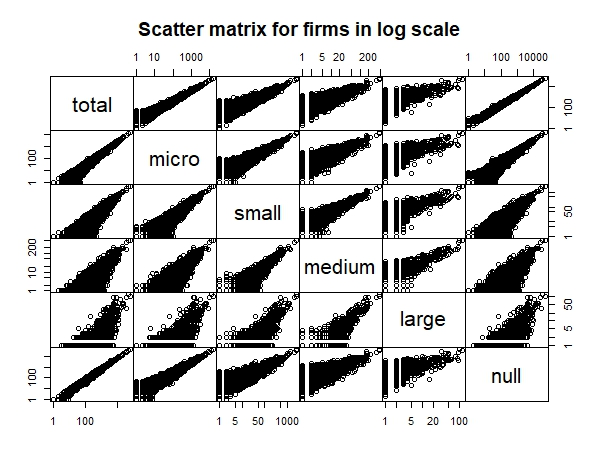
\includegraphics[width=0.5\textwidth]{scatter_firms_log.jpeg}}
	\subfloat{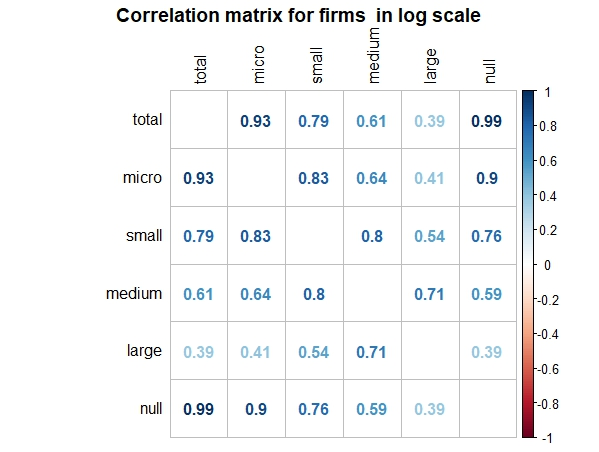
\includegraphics[width=0.5\textwidth]{corr_firms_log.jpeg}}
\end{figure}
Including Paris
\end{frame}


\begin{frame}{\textcolor{bscuro}{PCA}}
	Using original data scaled (not logs)
	
	Most typical vs. Excluding just Paris
	\begin{figure} 
		\centering
		\subfloat{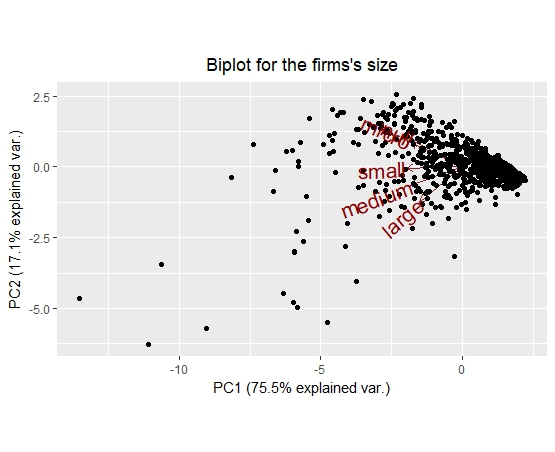
\includegraphics[width=0.5\textwidth]{biplot_firms.jpeg}}
				\subfloat{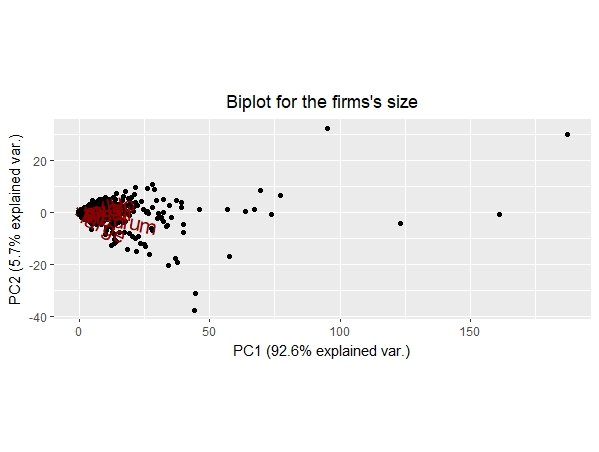
\includegraphics[width=0.5\textwidth]{biplot_firms_ParisExcl.jpeg}}
	\end{figure}
\end{frame}


\section{Summary}


\subsection{Problems encountered}


\begin{frame}{\textcolor{bscuro}{Issues}}
	\begin{itemize}
		\item Unique code for salary data 1/7 of the total 
		\item Loss of information when combining the separated datasets
		\item Missing additional information 
		\item French DOM-TOM regions
		\item Outliers and spatial correlation
	\end{itemize}
\end{frame}			


\subsection{Future works}


\begin{frame}{\textcolor{bscuro}{Future works}}
	%		Elaborate on future plans; can what you did during the course be the basis for a continuing project/collaboration? 
	\begin{itemize}
		\item Create meaningful indicators
		\item Take correlation into account (especially spatial)
		\item Perform clustering techniques to identify geographical clusters
		\item Perform groupwise lasso to predict salary data
		\item Verification/improvement of the obtained results 
		\item Compare the methodologies used with robust ones
		\item Find complementary datasets
	\end{itemize}	
\end{frame}		


\begin{frame}
	\centerline{\Huge\textcolor{bscuro}{ -- \emph{Thank you} -- }}
\end{frame}


\end{document}
